\documentclass[conference]{IEEEtran}
\IEEEoverridecommandlockouts
% The preceding line is only needed to identify funding in the first footnote. If that is unneeded, please comment it out.
\usepackage{cite}
\usepackage{amsmath,amssymb,amsfonts}
\usepackage{algorithmic}
\usepackage{graphicx}
\usepackage{textcomp}
\usepackage{xcolor}
\def\BibTeX{{\rm B\kern-.05em{\sc i\kern-.025em b}\kern-.08em
    T\kern-.1667em\lower.7ex\hbox{E}\kern-.125emX}}
\begin{document}

\title{CENG466, Fall 2022, THE 3\\

}

\author{\IEEEauthorblockN{1\textsuperscript{st} Fırat Ağış}
\IEEEauthorblockA{\textit{Department of Computer Engineering} \\
\textit{Middle East Technical University}\\
Ankara, Turkey \\
e2236867@ceng.metu.edu.tr}
\and
\IEEEauthorblockN{2\textsuperscript{nd} Robin Koç}
\IEEEauthorblockA{\textit{Department of Computer Engineering} \\
\textit{Middle East Technical University}\\
Ankara, Turkey \\
e2468718@ceng.metu.edu.tr}
}

\maketitle

\begin{abstract}

\end{abstract}

\begin{IEEEkeywords}

\end{IEEEkeywords}

\section{Face Detection}
For face detection, we propose an algorithm that use k-means to separate color groups, chooses the color group that is most likely to include skin colors and then uses morphological operations and convolution operation to detect areas that are most likely to include faces in the image. Our algorithm posses 3 distinct stages:
\begin{enumerate}
	\item \textit{Preprocessing:} Process the image to be more suitable for our algorithm and performs some processes to make the algorithm run a lot faster.
	\item \textit{K-Means:} Using k-means algorithm with randomized starting means to detect the pixels that are most likely to be in the color of skin tones.
	\item \textit{Context Based Postprocessing:} Using morphological operations and convolution operation to detect which clusters of the pixels that are found in the previous step to be the part of a face.
\end{enumerate}
\subsection{Preprocessing}
\begin{figure}[h]
    \centering
    \includegraphics[width=0.4\textwidth]{resources/non-equal vs equal.jpg}
    \caption{Difference in final results, on left, without histogram equalization and on right, with histogram equalization}
    \label{fig:equal}
\end{figure}
\begin{enumerate}
	\item \label{step:A1} We first read the relevant image. Shown in Row 1 of Figure \ref{fig:pro1}.
	\item \label{step:A2} (Optional) We perform histogram equalization to differentiate skin tones from similar colors in the image, most notably, the leaves in the 1\_source.png and shirt and hair in 3\_sources.png. Its effectiveness in demonstrated in Figure \ref{fig:equal}. Shown in Row 2 of Figure \ref{fig:pro1}.
	\item \label{step:A3} (Optional) We down-sampled the 2\_source.png by a factor of 9 in order to complete the algorithm in a reasonable time. 
	\item \label{step:A4} We bit-sliced all images, eliminating the least significant bit. Colors that are differentiated by a single bit are most likely to be in the same color group, meaning this operation affected the quality of the k-means algorithm minimally while reducing the size of the color space by a factor of $2^3=8$. Shown in Row 3 of Figure \ref{fig:pro1}.
\end{enumerate}
\subsection{K-Means}
\begin{figure}[h]
    \centering
    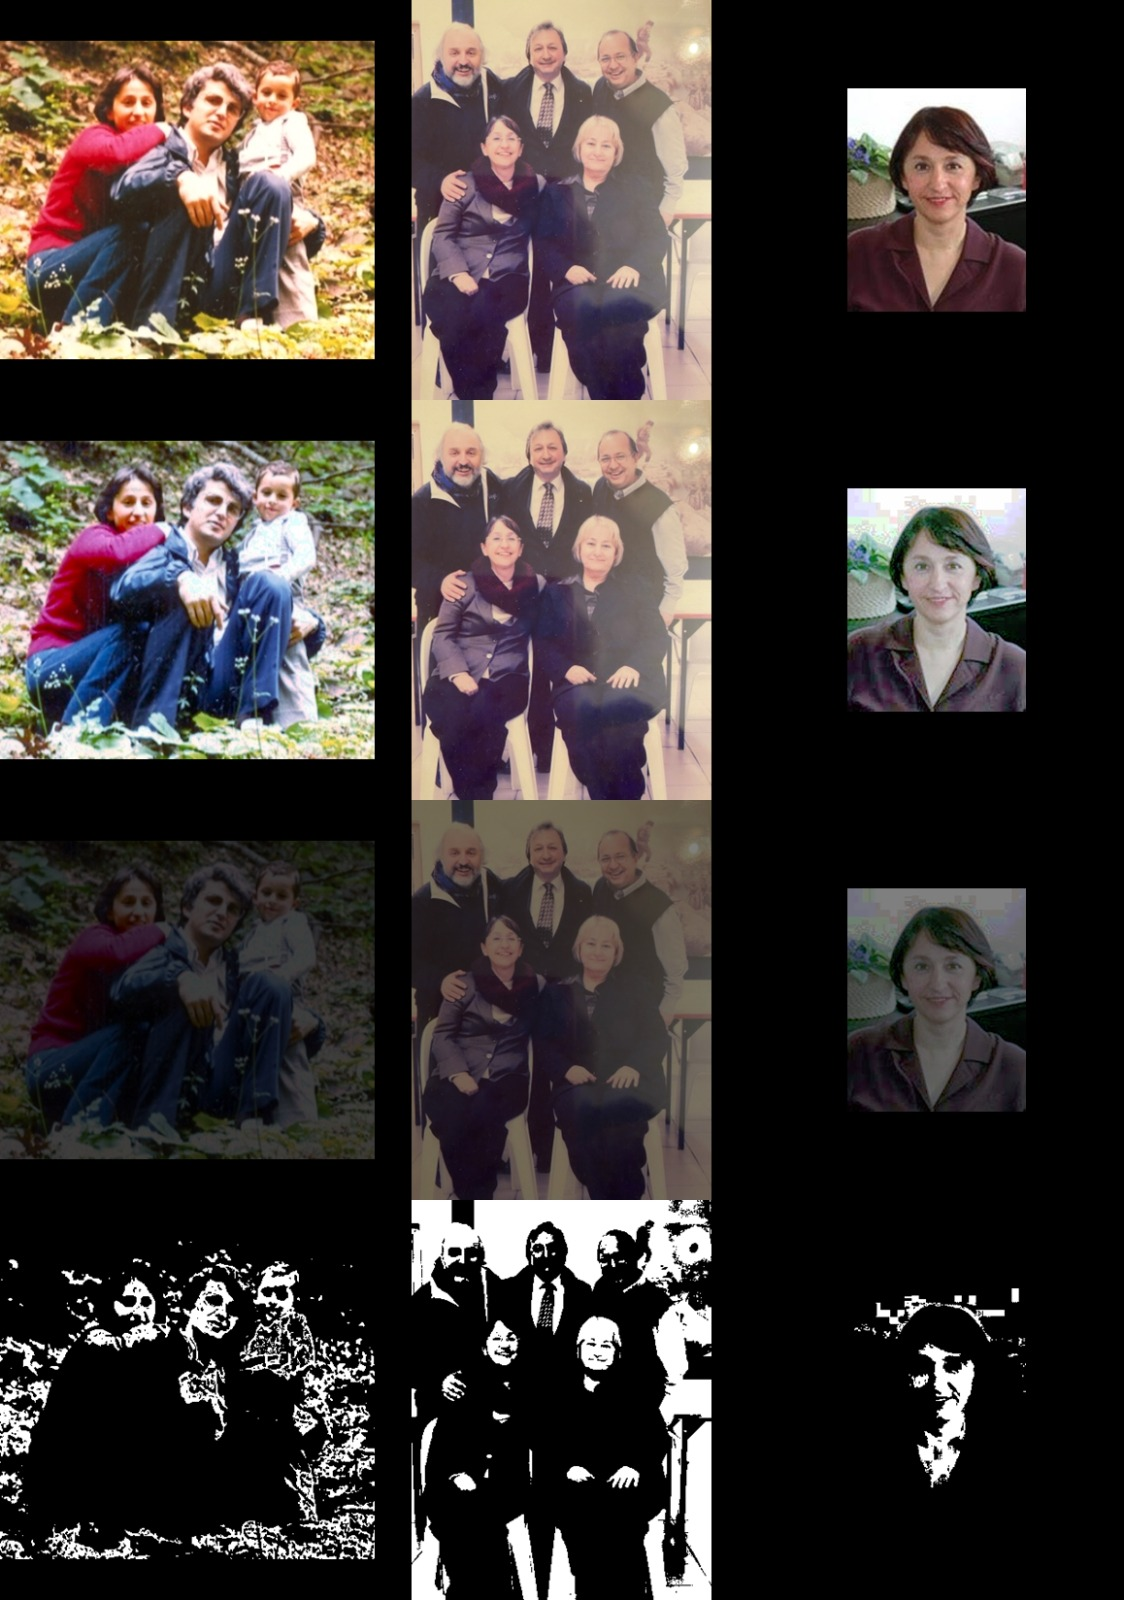
\includegraphics[width=0.4\textwidth]{resources/Progress 1.jpeg}
    \caption{Face detection progress for preprocessing and k-means stages}
    \label{fig:pro1}
\end{figure}
\begin{enumerate}
	\item \label{step:B1} We performed k-means algorithm with randomized initial means, acquiring means and colors closest to that means.
	\item \label{step:B2} We only took the colors whose means have the greatest red component using the knowledge that all faces are reddish in the context of color space.
	\item \label{step:B3} We eliminated any colors whose red component is less then their blue or green component using the same logic as the previous step. Shown in Row 4 of Figure \ref{fig:pro1}.
\end{enumerate}

\subsection{Context Based Postprocessing}
\begin{figure}[h]
    \centering
    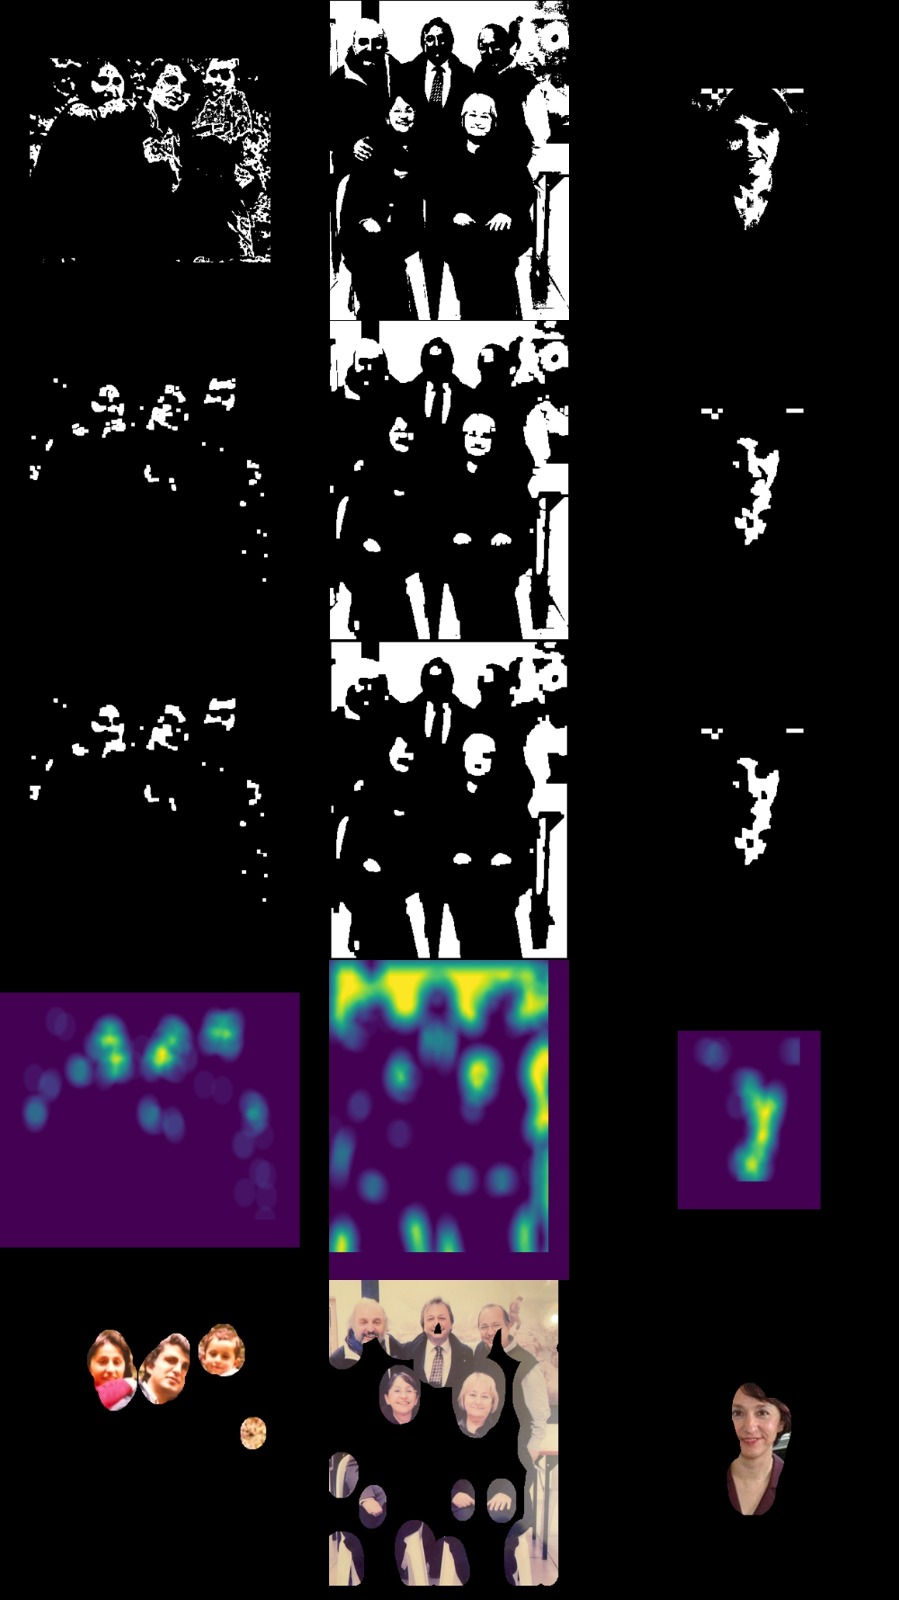
\includegraphics[width=0.4\textwidth]{resources/Progress 2.jpeg}
    \caption{Face detection progress for postprocessing stage}
    \label{fig:pro2}
\end{figure}
\begin{enumerate}
	\item \label{step:C1} (Optional) While processing 1\_source.png and 3\_sources.png, we used the assumption of faces being the central focus of images to eliminate pixels on the outer parts of the image. Shown in Row 1 of Figure \ref{fig:pro2}.
	\item \label{step:C2} We used opening operation with a 5x5 element to eliminate noise from the image. Shown in Row 2 of Figure \ref{fig:pro2}.
	\item \label{step:C3} We used closing operation with a 5x5 element to fix regions that are broken up during the previous step. Shown in Row 3 of Figure \ref{fig:pro2}.
	\item \label{step:C4} We used convolution with a elliptical mask, mimicking the shape of he face to determine locations where a face may lie. Shown in Row 4 of Figure \ref{fig:pro2}.
	\item \label{step:C5} We used thresholding to the result of the convolution, including the parts of the image that passed the tresholding, concluding the algorithm. Shown in Row 5 of Figure \ref{fig:pro2}.
\end{enumerate}
\subsection{Design Process}
After the implementation of basic k-means algorithm, execution time of the algorithm limited the speed of our further progress by trying different processes. For that reason, we implemented the preprocessing steps \ref{step:A3} and \ref{step:A4}.

Then we looked at commonalities between regions that make up the face, which brought us the reasoning we used in the k-means steps \ref{step:B2} and \ref{step:B3}.

After that, we experimented with histogram equalization to differentiate colors easier, giving us the results demonstrated in Figure \ref{fig:equal} in the final product.

When we arrived at the final result of k-means, given in Row 4 of Figure \ref{fig:pro1}, we determined the noise created by similarly colored regions to be a problem. To solve it, we implemented opening and closing mentioned in the postprocessing steps \ref{step:C2} and \ref{step:C3}. For the noise not eliminated by these steps, around the edge of the image for 1\_source.png, we implemented the postprocessing step \ref{step:C1}.

Morphological operations didn't eliminated all non-face regions. To distinguish regions that are face shaped from others, we finally implemented the postprocessing steps \ref{step:C4} and \ref{step:C5}.
\subsection{Results}
\begin{figure}[h]
    \centering
    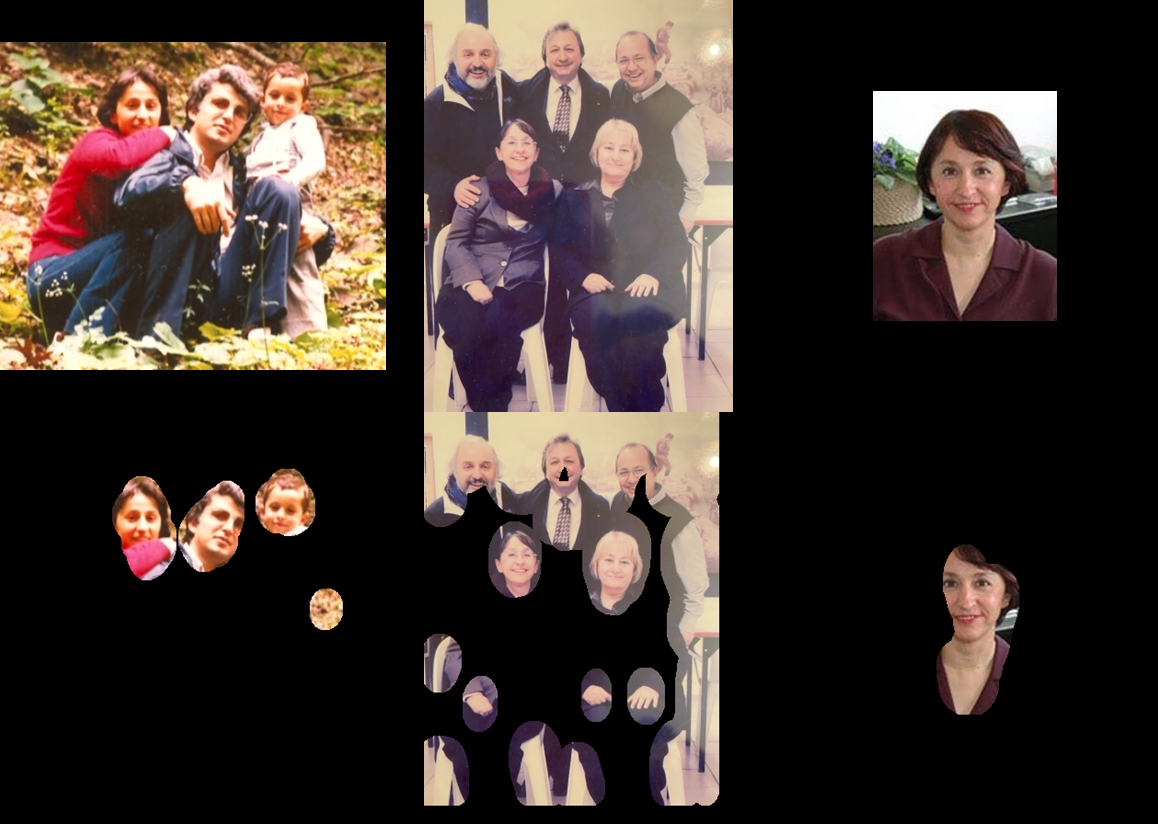
\includegraphics[width=0.4\textwidth]{resources/End Result Compare.jpeg}
    \caption{Original images and the end products}
    \label{fig:end}
\end{figure}
\section{Pseudo-coloring}

\section{Dependencies}
We used following libraries for the described reasons.
\begin{itemize}
	\item \textbf{os:} Handling non-existent input or output paths.
	\item \textbf{math:} Performing square root operation.
	\item \textbf{numpy:} Executing array and matrix operations.
	\item \textbf{PIL:} Reading images and converting them to arrays.
	\item \textbf{mathplotlib:} Creating histograms as graphics and writing arrays as image files.
\end{itemize}

\end{document}
